\subsection{Level2.1: $y=x^2$ について}
\subsubsection{プログラムソース(変更部分)}
\begin{breakbox}
\begin{verbatim}
行数 変更点
8  #define Y_MIN 0.0   /* 定義域の最小値 */
35 z = x * x;
47 z_dx = 2*x;
\end{verbatim}
\end{breakbox}

\subsubsection{観察意図と観察方法}
seedとalphaの2つのパラメータがあるため,alphaの値を固定し,seedの値を変化させる実験と
seedの値を固定し,alphaの値を変化させる実験の2つを行い,step数,探索の推移を観察する.

また,step数を観察する際にrun\_ave.shを用いて行い,探索の推移を観察をする際にtrans\_step\_vs\_func.shとtrans\_x\_vs\_func.sh,
trans\_x\_vs\_func\_seed1-10.shを用いて行った.\\

\begin{enumerate}
	\item  alphaの値を固定し,seedの値を変化させる実験\\
		観察したseed値は,1〜10までの小さい場合と,1000,2000,...100000の大きい場合の観察を行った.この際,alphaは0.1で固定している.
	\item seedの値を固定し,alphaの値を変化させる実験\\
		観察してalpha値は,0.1から0.9までの範囲の観察を行った,この時seed値は1で固定
\end{enumerate}

\subsubsection{実行結果}
実験1では,step数が少なくなっていってある程度低くなるとまた徐々に高くなるという波のような変化している.
実験2では,step数に大きな変化は起きなかったが探索の推移を観察より.
探索の初期位置が大きく変わっていることがわかった.
また,変化がalphaと類似していた(図\ref{trans_seed})

\begin{figure}[ht]
 \begin{center}
  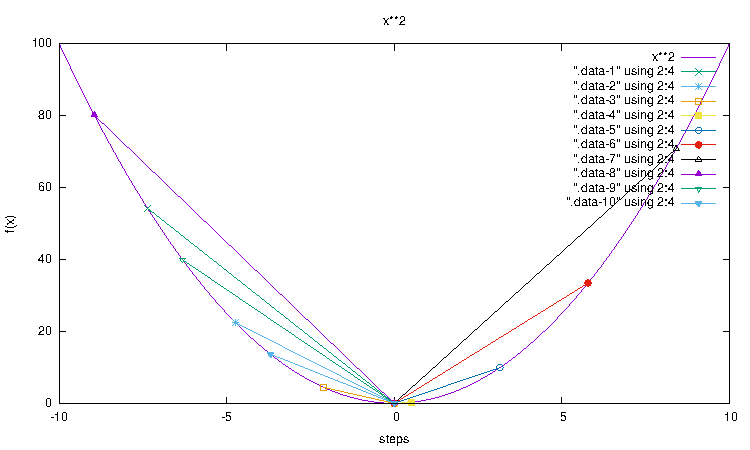
\includegraphics[width=10.0cm]{figs/level2.1/trans_seed1-10.pdf}
  \caption{探索初期値の変化}
	\label{trans_seed}
 \end{center}
\end{figure}
この図は,seed値を1〜10まで変化させ,それぞれの初期探索位置をグラフ化したものである.このとき,初期探索位置がわかりやすいように,探索回数の少ないalphaを使用している.

\subsubsection{考察}
結果より,alphaの値を変動させることによって,step数を大きく変動させることができることがわかった.\\
効率を考えると,探索回数が1000回と限られているため,できるだけ早く最小値を求めることが望ましいと考える.\\
だが,解の質を考えた場合,
すぐに0に収束してしまうため情報として最小値だけになってしまい情報量が少ない.
step数を多くすると探索の推移が細かに把握できるため,その分情報量が大きくなり,解の質としては向上すると考えた.  

